%!TEX root = ../main.tex

\section{Ferrimagnets: Fe$_{1-x}$Gd$_x$ samples}
\label{sec:ferrimagnets}

Lastly, layered systems of Iron (Fe) and Gadolinium (Gd) are tested for their
magnetic properties. Several samples with varying Gd-concentrations of $x\,\%$ are 
available to be experimented on. Unfortunately only one of the samples ($\#6$)
delivered physically sensible data at the time of the experiment. As a consequence, 
only the set of measurements pertaining to this sample will be analysed in depth.

In order to find the compensation temperature of the ferrimagnet, the sample is 
placed on a heating module whose temperature can be controlled by adjusting the 
applied voltage. Due to large fluctuations in temperature during measurements, the 
uneven contact of the sample to the heating element as well as other environmental 
factors, the temperature of the sample is assumed to have an uncertainty of 
$\pm\SI{1}{\celsius}$. After the hysteresis at a specific temperature is measured,
the temperature of the sample is changed and the process is repeated for a different
temperature. The results of this survey are fitted to the theoretical model 
introduced in \autoref{sec:ferromagnet}. The gathered model parameters are presented 
in \autoref{tab:fitvals-ferri}. A selected few measurement are also visualised in 
\autoref{fig:ferrimagnet-measurement}. As can be seen in both the table and the
figure, the coercive field strength ($H_c$) decreases with increasing temperature.

\begin{figure}
	\centering
	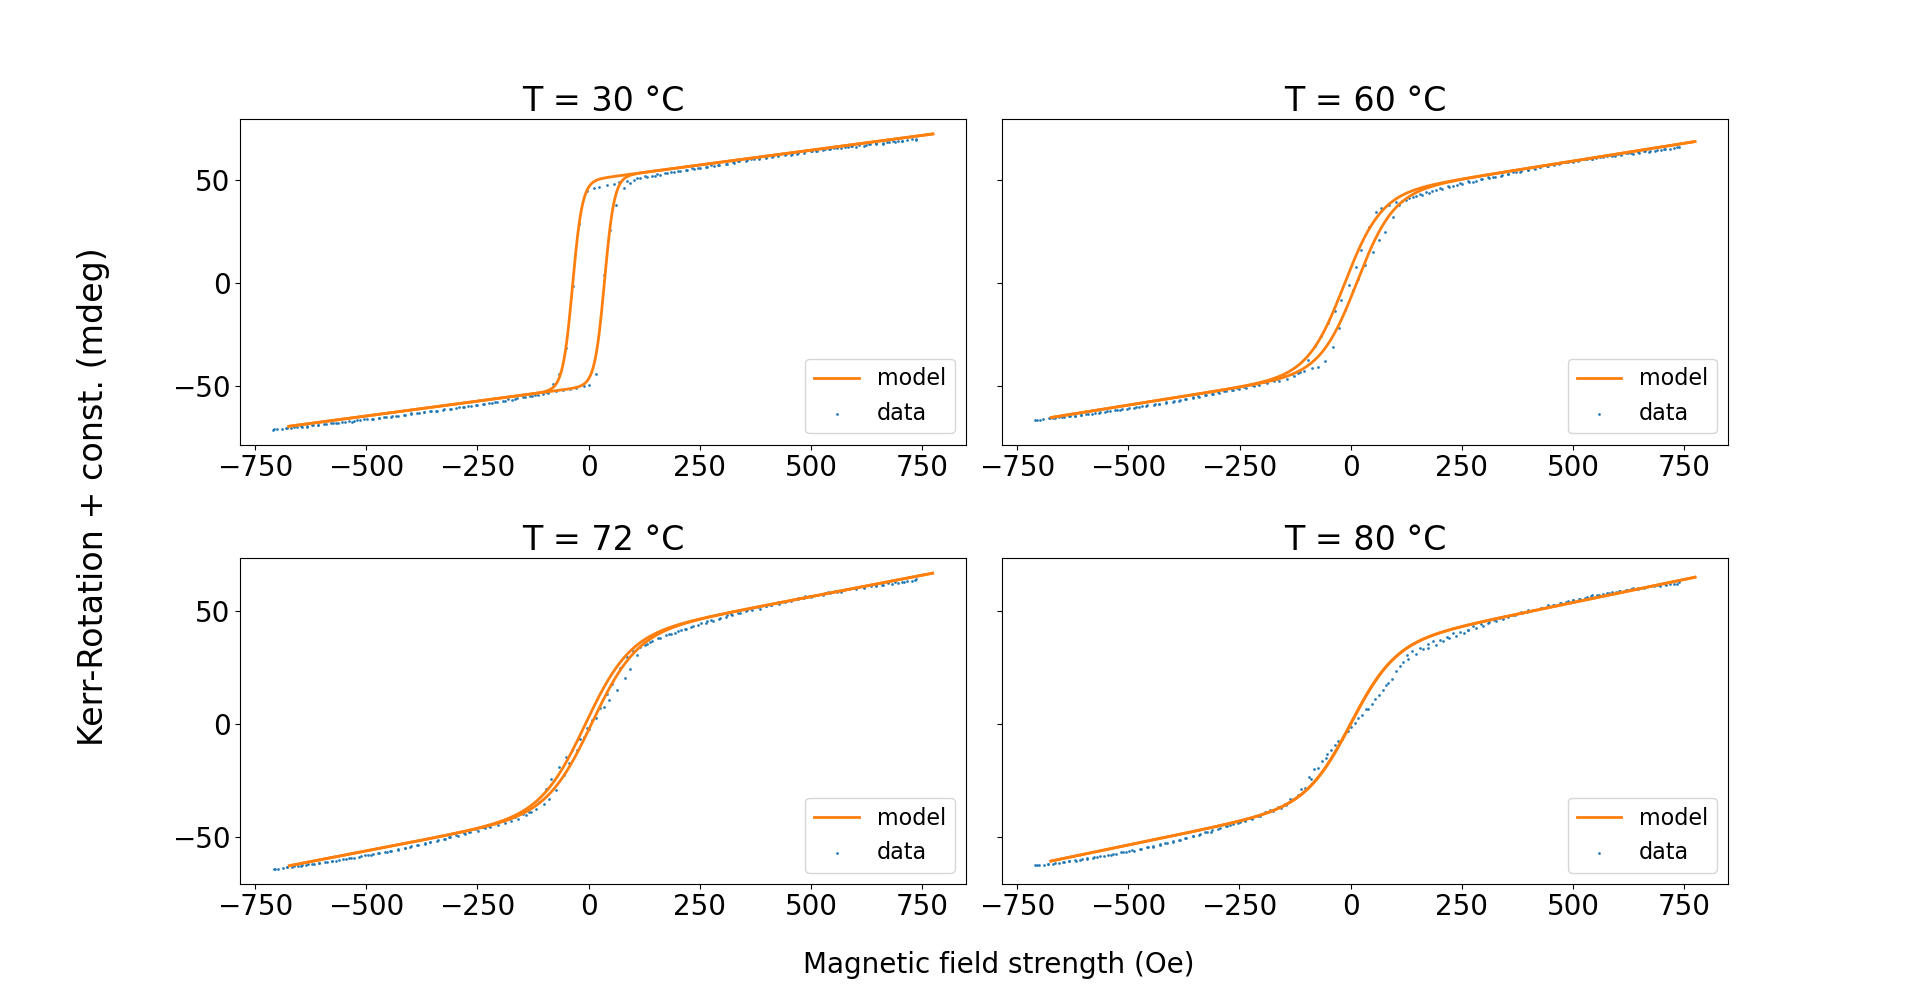
\includegraphics[width=1.0\textwidth]{./fig/ferrimagnet_measurement.png}
	\caption{The hysteresis of a FeGd layer system for different temperatures}
	\label{fig:ferrimagnet-measurement}
\end{figure}



\begingroup
\renewcommand{\arraystretch}{1.1}
\begin{table}
	\begin{center}
	\caption{Hysteresis best fit values for different magnet temperatures. Statistical errors estimated by the fitting algorithm are again neglected due to their small relative sizes.}
	\begin{tabular*}{\textwidth}{@{\extracolsep{\fill}} c|cccc}
  \toprule
	\hline
  $d$ & $\Upphi_s$ & $A$ & $H_c$ & $\mu$ \\
	\hline
  \SI{00}{\degree\celsius} & \SI{58.6761}{\milli\degree & \SI{149.7627}{\per\milli\oersted} & \SI{94.93}{\oersted} & \SI{26.36}{\micro\degree\per\oersted} \\
  \SI{10}{\degree\celsius} & \SI{55.2614}{\milli\degree & \SI{123.4514}{\per\milli\oersted} & \SI{69.87}{\oersted} & \SI{25.02}{\micro\degree\per\oersted} \\
  \SI{20}{\degree\celsius} & \SI{53.0343}{\milli\degree & \SI{68.1633}{\per\milli\oersted} & \SI{50.90}{\oersted} & \SI{26.50}{\micro\degree\per\oersted} \\
  \SI{30}{\degree\celsius} & \SI{50.1260}{\milli\degree & \SI{45.6059}{\per\milli\oersted} & \SI{35.93}{\oersted} & \SI{28.72}{\micro\degree\per\oersted} \\
  \SI{40}{\degree\celsius} & \SI{47.5209}{\milli\degree & \SI{26.9361}{\per\milli\oersted} & \SI{25.27}{\oersted} & \SI{30.24}{\micro\degree\per\oersted} \\
  \SI{50}{\degree\celsius} & \SI{45.1964}{\milli\degree & \SI{18.8061}{\per\milli\oersted} & \SI{19.83}{\oersted} & \SI{32.16}{\micro\degree\per\oersted} \\
  \SI{60}{\degree\celsius} & \SI{41.9797}{\milli\degree & \SI{12.2294}{\per\milli\oersted} & \SI{14.17}{\oersted} & \SI{34.46}{\micro\degree\per\oersted} \\
  \SI{70}{\degree\celsius} & \SI{38.8206}{\milli\degree & \SI{10.0000}{\per\milli\oersted} & \SI{9.60}{\oersted} & \SI{36.90}{\micro\degree\per\oersted} \\
  \SI{72}{\degree\celsius} & \SI{37.3744}{\milli\degree & \SI{10.0000}{\per\milli\oersted} & \SI{7.47}{\oersted} & \SI{37.96}{\micro\degree\per\oersted} \\
  \SI{75}{\degree\celsius} & \SI{37.2512}{\milli\degree & \SI{10.0000}{\per\milli\oersted} & \SI{6.18}{\oersted} & \SI{38.06}{\micro\degree\per\oersted} \\
  \SI{80}{\degree\celsius} & \SI{33.3113}{\milli\degree & \SI{10.0000}{\per\milli\oersted} & \SI{-0.51}{\oersted} & \SI{40.87}{\micro\degree\per\oersted} \\
	\hline
	\bottomrule
	\end{tabular*}
	\label{tab:fitvals-ferro}
	\end{center}
\end{table}
\endgroup


